\documentclass[11pt,a4paper]{article}
\usepackage[latin1]{inputenc}
\usepackage{amsmath}
\usepackage{amsfonts}
\usepackage{amssymb}
\usepackage{array}
\usepackage{graphicx}
\author{Jordan Murray}
\title{EECS305 Lab5}
\begin{document}
\begin{center}
\fontsize{24}{12}\selectfont
\textbf{Experiment 3: Model Identification and Transient Response of a DC Servo Motor System }
\end{center}

\section{OBJECTIVES:}
\begin{itemize}
\item To model and identify some of the parameters of a DC servo motor system.
\item To illustrate the basic idea of closed-loop feedback control.
\item To illustrate the transient response of a second order system to a step input and find the relationship between the parameters of the transient response and the parameters of the closed-loop DC motor system.
\end{itemize}


\section{BASIC KNOWLEDGE}
In this experiment we introduce mathematical models for a DC servomechanism and basic identification methods.

A block diagram for a typical servomechanism is shown in Fig. ~\ref{fig:servoblock}.  The action of the servomechanism is to track a desired position (or speed) despite the 
presence of disturbance inputs to the process and despite errors in the 
sensor data.

\begin{figure}[here]
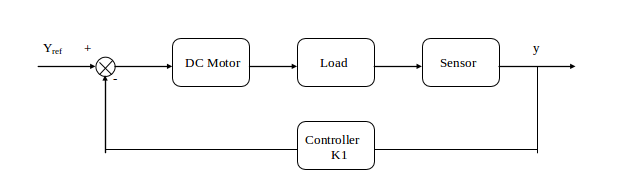
\includegraphics[width=\textwidth]{imglab/servoblockdiagram.png}
\caption{Servomechanism block diagram}
\label{fig:servoblock}
\end{figure}

\subsection{Model Development}
\begin{figure}[here]
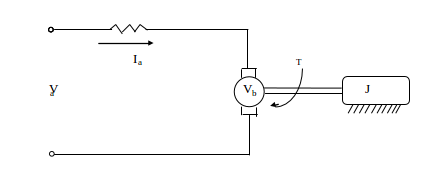
\includegraphics[width=\textwidth]{imglab/servoschemdiagram.png}
\caption{schematic diagram of the DC servo motor}
\label{fig:servoschem}
\end{figure}

We begin by developing a simplified linear model of an armature controlled DC servo motor and load. Fig. ~\ref{fig:servoschem} shows the schematic diagram of the motor and load.

Neglecting the inductance of the armature circuit, the armature voltage V$_{a}$ produces a current I$_{a}$ as given by:

\begin{equation} \label{eq:1}
I_{a} = \frac{V_{a}-V_{b}}{R_{a}}
\end{equation}

Here V$_{b}$ denotes the back emf of the motor and R$_{a}$ is the armature resistance.

The motor torque T is proportional to I$_{a}$:

\begin{equation} \label{eq:2}
T = K_{T}I_{a}
\end{equation}

But from Newton's law, assuming an inertia load:

\begin{equation} \label{eq:3}
T = J\ddot{\theta}
\end{equation}

combining equations \ref{eq:1}, \ref{eq:2}, and \ref{eq:3} we obtain:

\begin{equation} \label{eq:4}
K_{T}\left[\frac{V_{a}-V_{b}}{R_{a}}\right] = J\ddot{\theta}
\end{equation} 

Using the relationship V$_{b}$ = K$_{b}\dot{\theta}$ and, letting V$_{a}$ = U (input signal), we have:

\begin{equation} \label{eq:5}
\frac{K_{T}}{R_{a}}\left[U-K_{b}\dot{\theta}\right] = J\ddot{\theta}
\end{equation}

\begin{equation} \label{eq:6}
\frac{JR_{a}}{K_{T}}\ddot{\theta}+ K_{b}\dot{\theta} = U
\end{equation}

\begin{equation} \label{eq:7}
\ddot{\theta} + \frac{K_{b}K_{T}}{JR_{a}}\dot{\theta} = \frac{K_{T}}{JR_{a}}U
\end{equation}

or letting $\omega$ = $\dot{\theta}$, and 

\begin{equation} \label{eq:8}
\dot{\omega} + \frac{K_{b}K_{T}}{JR_{a}}\omega = \frac{K_{T}}{JR_{a}}U
\end{equation}

Equations \ref{eq:7} and \ref{eq:8} are the differential equations for the DC motor.

Let $\frac{K_{b}K_{T}}{JR_{a}} = \frac{1}{\tau}$, $\frac{K_{T}}{JR_{a}} = \frac{K_{0s}}{\tau}$. Here, $K_{0s}$ is the static gain and $\tau$ is the time constant of the system from input voltage to output speed. From D.E. \ref{eq:7} we can have the following transfer function:

\begin{equation} \label{eq:9}
\frac{\theta(s)}{U(s)} = \frac{K_{0s}}{s(\tau s + 1)}
\end{equation}

And from D.E. \ref{eq:8} we obtain the transfer function of the DC motor from U to $\dot{\theta}=\omega$:

\begin{equation} \label{eq:10}
\frac{\omega (s)}{U(s)} = \frac{K_{0s}}{(\tau s + 1)}
\end{equation}

Considering the measurements of speed and position, the system can be depicted as in Fig. ~\ref{fig:servomeasschem}

\begin{figure}[here]
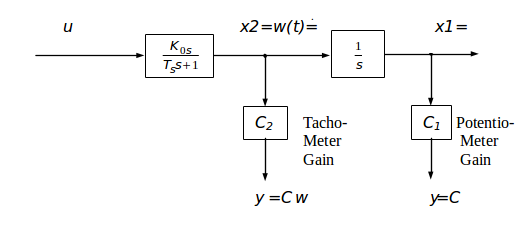
\includegraphics[width=\textwidth]{imglab/servomeasurementschematic.png}
\caption{schematic of the DC motor system with measurements}
\label{fig:servomeasschem}
\end{figure}

Then, the second order D.E. of the DC motor can be rewritten in the state-space format:

$x = A\dot{x} + Bu$
$y = Cx$

where, $x = \left[\begin{matrix}x_{1} \\ x_{2}\end{matrix}\right]$, $u=u$, $y = \left[\begin{matrix}y_{1} \\ y_{2}\end{matrix}\right]$, and
$A = \left[\begin{matrix}0 & 1 \\ 0 & -\frac{1}{\tau}\end{matrix}\right]$, $B=\left[\begin{matrix} 0 \\ \frac{K_{s}}{\tau} \end{matrix}\right]$, $C = \left[\begin{matrix}C_{1} & 0 \\ 0 & C_{2} \end{matrix}\right]$

Further, the input/output transfer function of the DC motor is:

\begin{equation} \label{eq:11}
G(s)=\frac{Y(s)}{U(s)} = \left[ \begin{matrix} G_{1}(s) \\ G_{2}(s) \end{matrix} \right] = \left[ \begin{matrix} \frac{C_{1}K_{0x}}{s(\tau s + 1)} \\ \frac{C_{2}K_{0s}}{\tau s + 1} \end{matrix} \right] = \left[ \begin{matrix} \frac{\left(\frac{C_{1}}{C_{2}}\right)*C_{2}K_{0s}}{s(\tau s + 1)} \\ \frac{C_{2}K_{0s}}{\tau s + 1} \end{matrix} \right]
\end{equation}

Define: $C_{s}=C_{1}/C_{2} and K_{s}=C_{2}K_{0s}$, then

\begin{equation} \label{eq:12}
G(s)=\frac{Y(s)}{U(s)} = \left[ \begin{matrix} G_{1}(s) \\ G_{2}(s) \end{matrix} \right] = \left[ \begin{matrix} \frac{C_{s}K_{s}}{s(\tau s + 1)} \\ \frac{K_{s}}{\tau s + 1} \end{matrix} \right]
\end{equation}

The model has one pole at the origin and one pole on the negative real axis. The problem is to identify parametesr $K_{s}, \tau$ and $C_{s}$. From \ref{eq:12}, the transfer function from input u to output $y_{2}$ is:

\begin{equation} \label{eq:13}
\frac{Y_{2}(s)}{U(s)} = \frac{K_{s}}{\tau s + 1}
\end{equation}

The step response of the first order system is shown in Fig. ~\ref{fig:servostepresp}:

\begin{figure}[here]
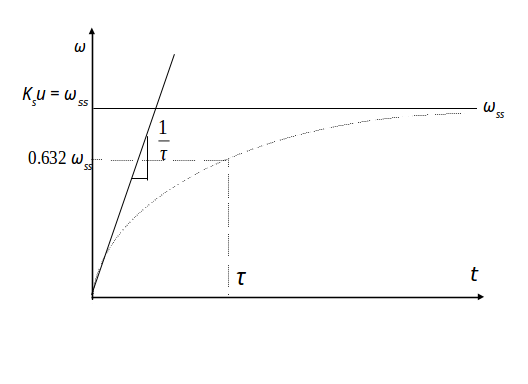
\includegraphics[width=\textwidth]{imglab/servostepresponse.png}
\caption{step response of the DC servo motor}
\label{fig:servostepresp}
\end{figure}

From this diagram, we can determine that the time constant of the motor, $\tau$, is the time it takes $y_{2}$ to reach 63.2\% of its steady state value $y_{2ss}$. We can also obtain the steady-state gain $K_{s} = \frac{y_{2ss}}{U_{ss}}$.

In addition, notice that regarding $C_{s}$ there is a conformity that has to be satisfied:

\begin{equation} \label{eq:14}
C_{s} = \frac{\frac{dy_{1}}{dt}}{y_2}
\end{equation}
This gives the way to identify $C_{s}$.

\subsection{Closed Loop Control for a DC servomechanism} \label{ss:closedloop}
The block diagram of Fig. ~\ref{fig:servoblock} for the servomechanism can be simplified into the block diagram given in Fig. ~\ref{fig:servotfblock}.

\begin{figure}[here]
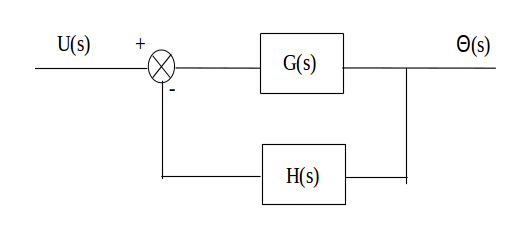
\includegraphics{imglab/servotfblock.png}
\caption{simplified block diagram}
\label{fig:servotfblock}
\end{figure}

This configuration is referred to as a negative feedback closed loop configuration where G(s) is the forward loop transfer function and H(s) is the feedback loop transfer function. The equivalent transfer function between the input r(t) and the output y(t) as shown in Fig. ~\ref{fig:servostepresp} can be represented as the transfer function G'(s) shown in Fig. ~\ref{fig:servocltfblock}.

\begin{figure}[here]
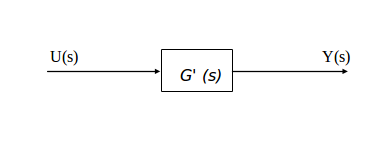
\includegraphics{imglab/servocltfblock.png}
\caption{eqivalent closed-loop transfer function}
\label{fig:servocltfblock}
\end{figure}

\begin{equation} \label{eq:15}
G'(s)=\frac{Y(s)}{U(s)}=\frac{G(s)}{1+G(s)H(s)}
\end{equation}

Considering the servomechanism transfer function:

From Eq. \ref{eq:9}: $G(s)=\frac{C_{s}K_{s}}{s(\tau s + 1)}$,

H(s) = K$_{1}$ (Output feedback controller gain),

\begin{equation} \label{eq:16}
G'(s)=\frac{\frac{C_{s}K_{s}}{\tau}}{s^{2} + \frac{s}{\tau} + \frac{K_{1}K_{s}C_{s}}{\tau}}
\end{equation}

We observe that the transfer function of the closed-loop system, G'(s) is a second order system with one free controller parameter $K_{1}$. Changing the gain $K_{1}$ can be used to alter the transient dynamics of the second order system.

\section{EXPERIMENTAL PROCEDURES:}
\subsection{Model Identification:}
\begin{enumerate}
\item Run \textbf{MATLAB} and open the model \textbf{Lab3\_identification.slx}. The \textit{DC servo} block contains a masked model of a DC servo motor. Run the model. A unit step input is applied to the motor winding at t = 1s. Open the scope and look at the angular velocity trace. Determine the steady-state speed of the motor. This is the value of $K_{s}$, the steady-state gain. Determine the time at which the speed reaches 63.2\% of its final value. Find the elapsed time since the step function was applied. This value is the time constant $\tau$.
\item Open the model \textbf{Lab3\_Comparison.slx}. Update the servo transfer function block to match the parameters you determined above. Compare the behavior of your model transfer function to that of the DC Servo block. See if you can more closely match the DC Servo block by making small changes in your transfer function parameters.
\end{enumerate}

\subsection{Transient Response:}
In this part the closed loop servomechanism system for position control is being implemented as explained in section ~\ref{ss:closedloop}. The main goal is to change the controller gain $K_{1}$, observe the characteristics of the transient response and relate these to the parameters of the closed-loop system and the parameters which define the transient response.
The following objectives should be met:
\begin{enumerate}
\item Understanding the relationship between the system parameters: damping ratio ($\zeta$) and natural frequency ($\omega_{n}$), the transient response parameters: \%overshoot ($M_{p}$), settling time ($T_{settling}$), peak time ($T_{p}$), rise time ($T_{r}$), and the closed-loop poles, with the gain $K_{1}$.

\item Understanding the qualitative effect of the controller gain $K_{1}$ on the transient response of the servomechanism.

\item Obtaining a basic understanding of computer control for the DC-servo system.
\end{enumerate}

Procedure:
\begin{enumerate}
\item Open the model \textbf{Lab3\_Transient.slx} and run it. Save the theta trajectories associated with each of the different values of $K_{1}$. You will need this data for an exercise.
\end{enumerate}

\section{EXERCISES:}
\begin{enumerate} 
\item \label{ex:maketable} Fill in the following table for each case.
\begin{center}
\begin{tabular}{|c|c|c|c|c|c|c|c|}
\hline
Gain & Poles & \%overshoot & $\zeta$ & $\omega_{n}$ & $T_{settling}$ & $T_{peak}$ & $T_{r}$ \\ \hline
\qquad \qquad & \qquad \qquad & \qquad \qquad & \qquad \qquad & \qquad \qquad & \qquad \qquad & \qquad \qquad & \qquad \qquad \\ \hline 
\qquad \qquad & \qquad \qquad & \qquad \qquad & \qquad \qquad & \qquad \qquad & \qquad \qquad & \qquad \qquad & \qquad \qquad \\ \hline 
\qquad \qquad & \qquad \qquad & \qquad \qquad & \qquad \qquad & \qquad \qquad & \qquad \qquad & \qquad \qquad & \qquad \qquad \\ \hline 
\qquad \qquad & \qquad \qquad & \qquad \qquad & \qquad \qquad & \qquad \qquad & \qquad \qquad & \qquad \qquad & \qquad \qquad \\ \hline 

\end{tabular}
\end{center}


\item \label{ex:plots} Using the table from exercise \ref{ex:maketable}, plot the following:
\begin{enumerate}
\item Poles in the s plane for all values of gain constant $K_{1}$.
\item The damping ratio vs. $K_{1}$.
\item \% overshoot vs. $\zeta$.
\item settling time, $T_{settling}$ vs. $\zeta$.
\end{enumerate}

\item Using the graphs from exercise \ref{ex:plots}, try to explain (qualitatively) the effect of changing $K_{1}$ on:
\begin{enumerate}
\item Poles of the closed-loop system
\item Overshoot of the closed-loop system
\item Settling time of the closed-loop system
\end{enumerate}

\end{enumerate}


\end{document}